\documentclass[crop,tikz,border=1px]{standalone}

\usepackage{color}
\newcommand{\red}[1]{\textcolor{red}{#1}}

\usetikzlibrary{arrows,positioning,scopes,automata,calc}

\begin{document}
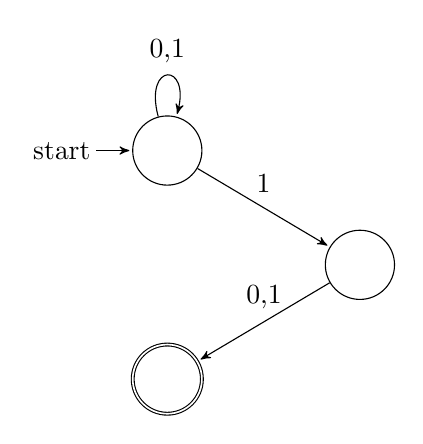
\begin{tikzpicture}[->,>=stealth',shorten >=1pt,auto,node
  distance=2cm,inner sep=2pt,minimum size=.6cm,
  mystate/.style={state,text centered}]

  \node[initial,mystate] (q0) {};
  \node[accepting,mystate] (q2) [below=of q0] {};
  \coordinate (mid) at ($(q0)!0.5!(q2)$);
  \node[mystate] (q1) [right=of mid] {};

  \path (q0) edge [loop above] node [above] {0,1} (q0)
        (q0) edge node [above] {1} (q1)
        (q1) edge node [above] {0,1} (q2);

\end{tikzpicture}
\end{document}
